\documentclass[a4paper,12pt,titlepage]{article}
\usepackage[pdftex]{graphicx}
\usepackage[headheight=15pt]{geometry}

\usepackage{fancyhdr}
\pagestyle{fancy}
\lhead{Exercises}
\chead{}
\rhead{GIS for Disease Outbreak Management}

\usepackage[english]{babel}									
\usepackage[utf8]{inputenc}	

\usepackage{array}
\usepackage{colortbl}

\usepackage[section]{placeins}
\usepackage{float}

%PDF hyperlinks
\usepackage[colorlinks=true,linkcolor=orange,citecolor=blue,bookmarksopen=true,bookmarksnumbered=true,pdfstartpage=1]{hyperref}
\hypersetup{
	pdftitle={GIS for Disease Outbreak Management},
	pdfauthor={Michael Wagner},
	pdfsubject={GIS for Disease Outbreak Management},
	pdfkeywords={GIS, QGIS, Disease Outbreak Management}
}

\usepackage[nonumberlist,nopostdot]{glossaries}
\setglossarystyle{alttree}
% Set max width of the abbreviation column
\glssetwidest{SWIO-RAFI-XX}

\makeglossaries
\loadglsentries{abbr}
\setacronymstyle{long-short}

\usepackage{color}
\definecolor{orange}{rgb}{1,.5,0}

\title{Exercises: GIS for Disease Outbreak Management}
\author{Michael Wagner (mwagner@allspatial.info)}
\date{July 12, 2016}     													

\clubpenalty=4500																
\widowpenalty=10000								
\linespread{1.3}

%%-------------------------Document begins--------------------------------------------
\begin{document}             											
\maketitle                   										

\tableofcontents
\listoffigures
\newpage
\printglossary[type=\acronymtype,title={List of Abbreviations}]
\newpage

\section{Animal disease outbreak management}

For this exercise it is assumed that you are familiar with basic \gls{gis} tasks and the concept of attribute and spatial queries as well as basic geoprocessing.

\subsection{Creating thematic maps showing the amount of livestock}

Open the \textit{vet.xslx} file that you will find in the \textit{Data/AgriData} directory of the \textit{GIS\_for\_Disease\_Outbreak\_Management} folder. Export the data of the three worksheets to a CSV (Comma Separated Value) file (three files all together). Open the resulting files with \textit{Notepad++} or \textit{Atom} and clean up the data. Remove any spaces from the parcel numbers and take care that only one parcel number is used per row/line. All parcel numbers must be in capital letters. The column names must not contain any spaces or special characters. Otherwise you cannot join the text files with the \textit{parcel} layer. If a semicolon (';') was used as the column separator replace it with a comma (','). Save the files.

Open a new QGIS project and load the \textit{parcel} and \textit{district} layers. Join the \textit{parcel} layer with the first CSV file (Figure \ref{fig:join2}).

\begin{figure}[htb]
	\centering
	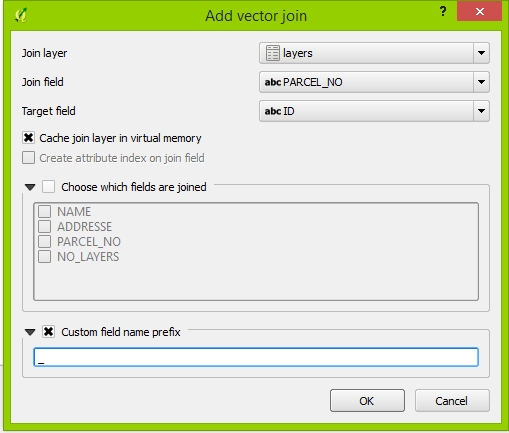
\includegraphics[width=8cm]{Images/join2.png}
	\caption{Performing an attribute join}\label{fig:join2}
\end{figure}

Perform an attribute query to select only those parcels that contain data from the CSV file. Save the selection as a new Shapefile. Remove the join from the parcel layer and add a new join with the next CSV file. Finally you should have three new Shapefiles:

\begin{itemize}
\item layers\_parcel
\item broilers\_parcel
\item fatners\_parcel
\end{itemize}

Create three thematic maps that show the parcels by the number of livestock. Give the original \textit{parcel} layer a decent and light color so that the parcels with livestock can easily be distinguished and spotted (Figure \ref{fig:layers_parcel}).

\begin{figure}[htb]
\centering
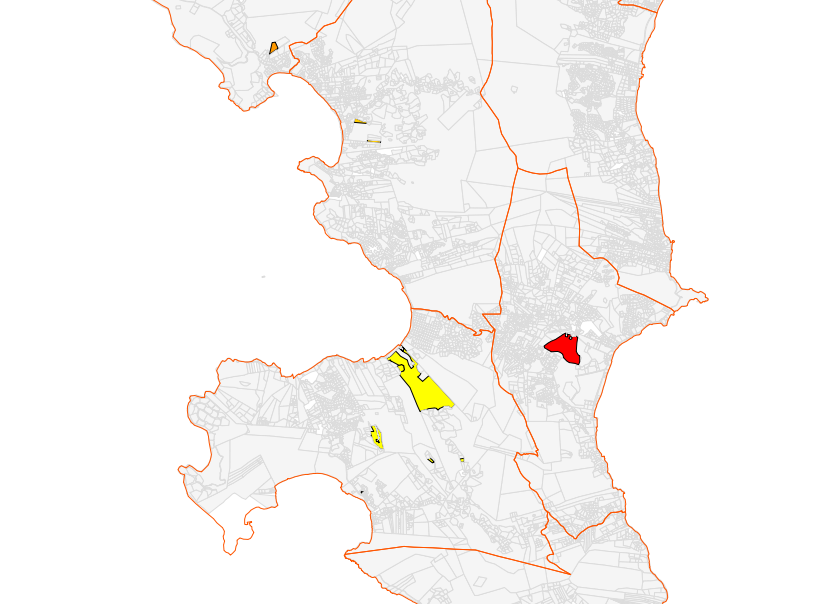
\includegraphics[width=12cm]{Images/layers_parcel.png}
\caption{Showing parcels with layers (chicken)}\label{fig:layers_parcel}
\end{figure}

\subsection{Capturing the outbreak location}
Let's assume an outbreak was reported and an inspector went to the reported site to confirm the suspicion and capture the location (GPS coordinate) of the outbreak. You find the captured outbreak location in the \textit{outbreak\_location\_gps.csv} file. Use the \textit{Add Delimited Text Layer} tool to load the outbreak location into QGIS. It might happen that you don't see any additional point on your existing map (with the parcels and districts). This is the case if you don't have \textit{on-the-fly} coordinate reference system transformation enabled in your \textit{Project Properties}. The coordinate of the outbreak location is in a coordinate reference system different from the one used by the two other layers. By default the GPS device records a coordinate in a geographic coordinate reference system (using longitude and latitude) while the current layers in QGIS use a projected coordinate system. We need to tell QGIS to do an on-the-fly transformation of the coordinates. From the \textit{Project} menu select \textit{Project Properties...} and open the \textit{Coordinate Reference System} tab. Toggle the \textit{on-the-fly} box as shown in Figure \ref{fig:on_the_fly} and select the (target) coordinate system with EPSG-ID 32740. That is the projected coordinate system for data on Mahe, Praslin and La Digue. As soon as you click the \textit{OK} button the location of the outbreak should appear as a point on a chicken farm in the South of Mahe.

\begin{figure}[htb]
\centering
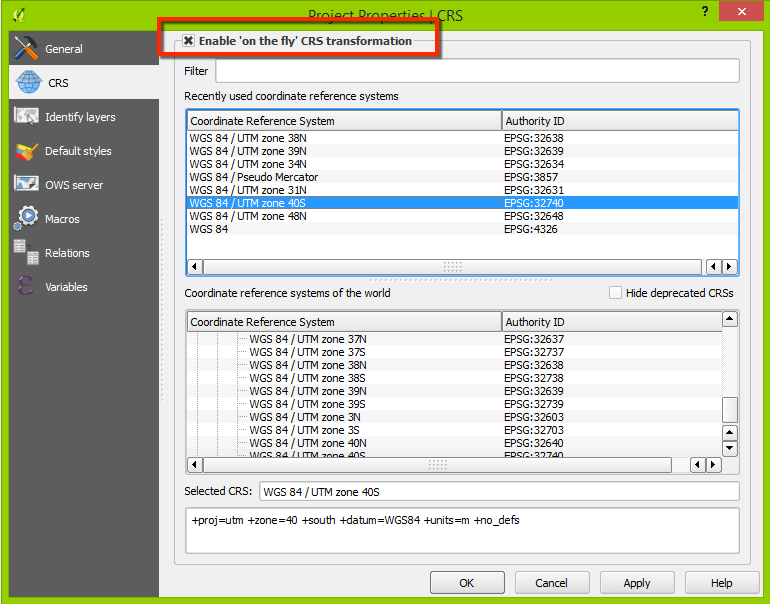
\includegraphics[width=12cm]{Images/on_the_fly.png}
\caption{Enabling on-the-fly transformation}\label{fig:on_the_fly}
\end{figure}

Create a new Shapefile \textit{outbreak\_location} and add some attributes you deem useful and important. Toggle editing for this layer and capture the outbreak location by snapping to the GPS point from the text file layer. Fill in the required attributes and save your edits. Remove the original layer of the outbreak location that you loaded from a CSV file, it is not needed anymore.

\subsection{Creating quarantine zones}
Depending on the rules (legislation?) defined for the case of an animal disease outbreak, quarantine zones will need to be established around the outbreak location. Let's assume that all animals within a 1km zone will need to be culled while the ones within 3km must be vaccinated and observed. Thus, the 3km zone will also be a surveillance zone. Create the two zones accordingly using the spatial capabilities of the GIS (\textit{Buffers} tool in this case). Make sure that the two zones have no intersection set. By default this is the case. You can use the \textit{Difference} tool (menu \textit{Vector:Geoprocessing Tools}) to create zones that do not intersect.

Find out which farms are in the quarantine zones and how much livestock will need to be culled or vaccinated. Use the \textit{Basic statistics} tool from the \textit{Vector:Analysis Tools} menu.

\subsection{Identifying the location for road barricades}
Any vehicle entering the 1km quarantine zone should be checked and disinfected. Identify where to put road control points/barricades accordingly. That would be the intersections of the roads with the boundary/outline of the 1km quarantine area. You will need to use two new tools to identify the location of control points, \textit{Polygons to lines} from the \textit{Vector:Geometry Tools} tools menu and \textit{Line intersections} from the \textit{Vector:Analysis Tools} menu. Convert the 1km-zone layer to a line layers. Calculate the intersections of the roads with the outline of the 1km zone (Figure \ref{fig:line_intersection}).

\begin{figure}[H]
	\centering
	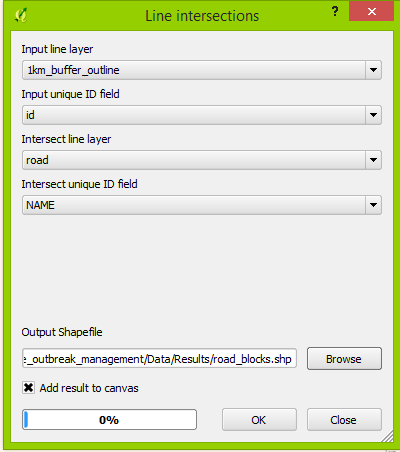
\includegraphics[width=6cm]{Images/line_intersection.png}
	\caption{Calculating line intersections}\label{fig:line_intersection}
\end{figure}

The result could look as in Figure \ref{fig:control_points}. In addition create a thematic map that shows the roads by road classes (main road, secondary, etc.). Such a map helps to identify the areas that can be reached easily by a car and those ones where access might be difficult (and an off-road car is needed).

\begin{figure}[htb]
\centering
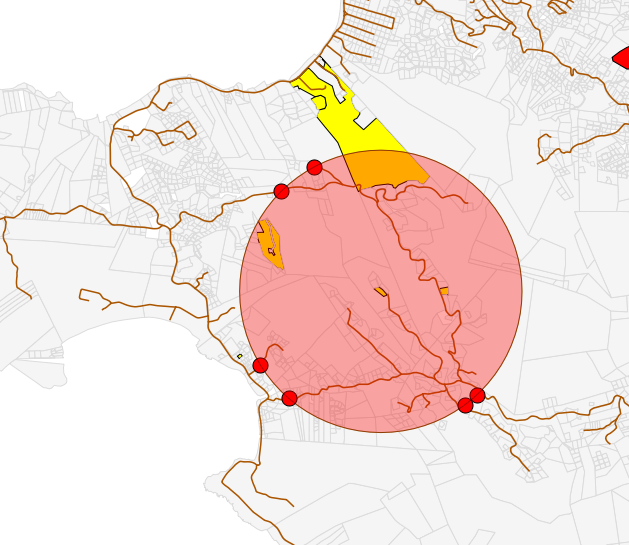
\includegraphics[width=12cm]{Images/control_points.png}
\caption{Identifying road control points}\label{fig:control_points}
\end{figure}

\subsection{Identifying the number of people in the outbreak neighbourhood}
Assuming that the animal disease is contagious also for human beings you need to identify the number of people under risk, especially those in the immediate neighbourhood of the outbreak location in the 1km zone. Load the \textit{ea\_mahe} Shapefile from the \textit{NBS} directory in the \textit{Data} folder. This Shapefile contains the boundaries of the Census EA units. The actual census data you will find in the \textit{CENSUS\_DATA.xlsx} file. Export that file to a CSV file and join it with the \textit{ea\_mahe} layer through the 4-digits EA ID. Save the result as a new Shapefile \textit{ea\_mahe\_final.shp}. Find those EAs that intersect with the 1km zone and use the \textit{Basic statistics} tool again to figure out the overall number of people living in that zone. Before using the \textit{Basic Statistics} tool set the total number of population to 0 for those EAs where no data is available (using the \textit{Field Calculator}). The \textit{Basic Statistics} tool does not like to work with NULL values (empty data).

\subsection{Identifying public facilities for evacuation purposes}
In case that a larger number of people needs to be evacuated from the 1km zone identify public facilities/premises within 3km of the outbreak location (but outside the 1km quarantine zone). These might need to be used to shelter quite a number of people for a period of time. Public premises could be churches and schools for example. Identify parcels in Baie Lazare with an area greater or equal than 3000 sqm. These could be used in addition to set up temporary shelter (tents/huts). Identify those buildings in Baie Lazare that are not within 1500 meters of any governmental hospital/clinic. Households there might have difficulties to reach medical care swiftly.

\section{Human disease outbreak management}

During the last months quite a few Dengue cases were reported in the Seychelles. For the purpose of this training data on these cases was provided by the \gls{dsru}. Load the files \textit{dengue\_cases\_32740.csv} and \textit{dengue\_cases\_4326.csv} into QGIS and assign the relating coordinate reference system. The files contain the location of each suspected case. Depending on the inspector who was recording the case the location was either provided in UTM coordinates or through Latitude/Longitude. Hence, two files are provided. Make sure you have \textit{on-the-fly} transformation enabled in the \textit{Project Properties} and set the coordinate reference system to EPSG:32740 (UTM Zone 40S). Save the CSV layer loaded from UTM coordinates to a new Shapefile named \textit{dengue\_cases}. In the CSV layer loaded from Lat/Lon coordinates select all points/locations and select \textit{Copy Features} from the \textit{Edit} menu. Toggle the editing mode for the \textit{dengue\_cases} layer (the Shapefile you just saved) and select \textit{Paste Features} from the Edit menu. Toggle editing again to leave the editing mode and save your changes. You should now have all Dengue cases in one single Shapefile layer in UTM coordinates. Remove the original CSV layers from the table of contents.

\subsection{Creating a heat map}

A heat map is used to visualise higher density of spatial features in a nice and easy-to-comprehend way. You will use it to visualise the concentration of Dengue cases. QGIS has a great heat-map style type already incorporated. Double-click the \textit{dengue\_cases} layer to open the \textit{Layer Properties} dialog and select the \textit{Style} tab. 

\begin{figure}[htb]
	\centering
	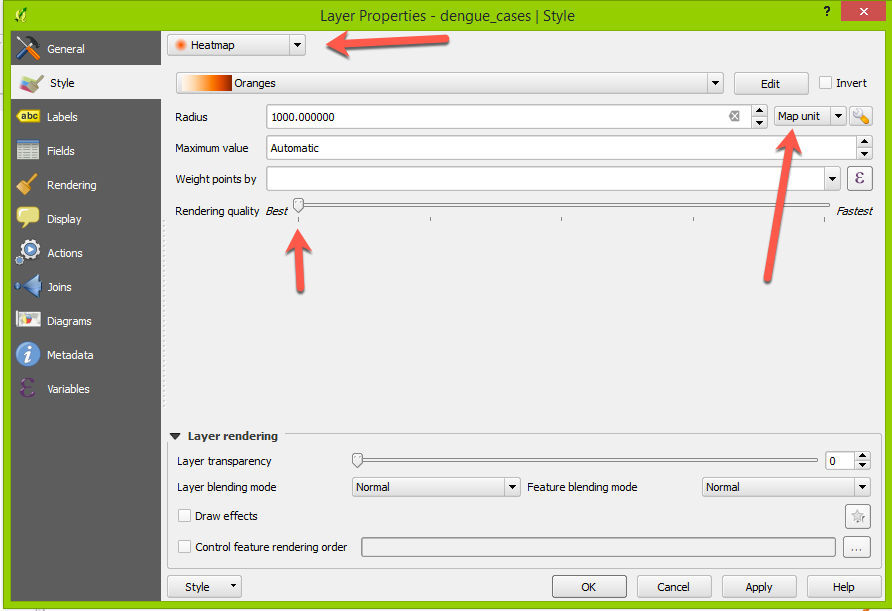
\includegraphics[width=12cm]{Images/heat_map_settings.png}
	\caption{Settings for heat map}\label{fig:heat_map_settings}
\end{figure}

Adjust the settings as shown in Figure \ref{fig:heat_map_settings}. Make sure to set the radius is set in \textit{Map Units}. Select a colour scheme of your choice and click OK.
Experiment with different settings for the radius and see how the map changes. A result could look like Figure \ref{fig:mahe_heat_map}.

\begin{figure}[htb]
	\centering
	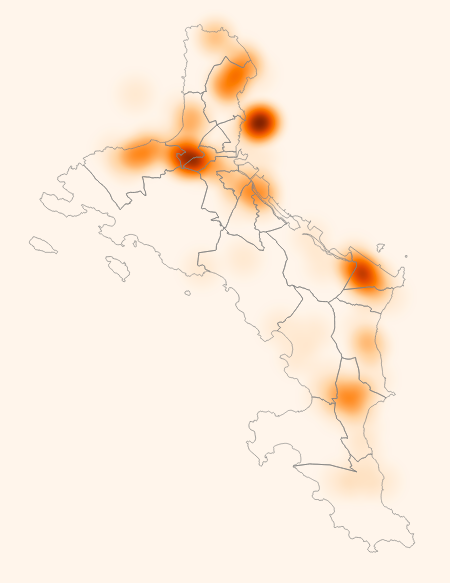
\includegraphics[width=8cm]{Images/mahe_heat_map.png}
	\caption{Heat map of Dengue cases on Mahe}\label{fig:mahe_heat_map}
\end{figure}

You could now try to find out if there is potential link of Dengue case to the location of wetlands. Go to the Working Group's data portal (\href{http://178.63.85.21}{Seychelles Datas Sharing}) and download the wetlands layer for Mahe as zipped Shapefile. Unzip the Shapefile, load it into QGIS and overlay it with the Dengue heat map. 

\subsection{Visualise change}

For a disease outbreak in particular it is useful to see the changes (spread or regression) throughout time. Unfortunately the data on Dengue cases that you received have no information on the date a case was reported or diagnosed. However, you can easily generate some mock data to simulate a potential scenario. Let's assume that all Dengue cases were reported between June 1 and 10, 2016. Double-click the \textit{dengue\_case} layer to open the \textit{Layer Properties} dialog. Select the \textit{Fields} tab and toggle the editing mode for the layer (by clicking on the button with a pencil icon). Select and delete the two columns \textit{E} and \textit{N}, you don't need them. Click on the last button on the toolbar to open the \textit{Field Calculator} (Figure \ref{fig:fields}). 

\begin{figure}[htb]
	\centering
	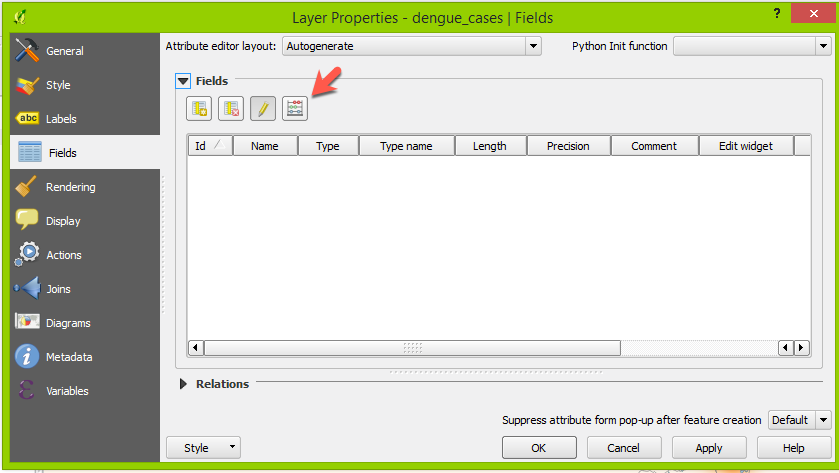
\includegraphics[width=12cm]{Images/fields.png}
	\caption{Opening the Field Calculator from the Layer Properties dialog}\label{fig:fields}
\end{figure}

In the \textit{Field Calculator} create a new field named \textit{reportdate} of data type \textit{Date}. In the Expression field enter the expression as shown in Figure \ref{fig:field_calc}. This will randomly create dates between June 1 and 10, 2016 for all dengue cases. Close the \textit{Field Calculator} by clicking OK and toggle the editing mode again in the \textit{Layer Properties} dialog to save your changes. Open the layer's attribute table to verify that the dates were generated as expected.

\begin{figure}[H]
	\centering
	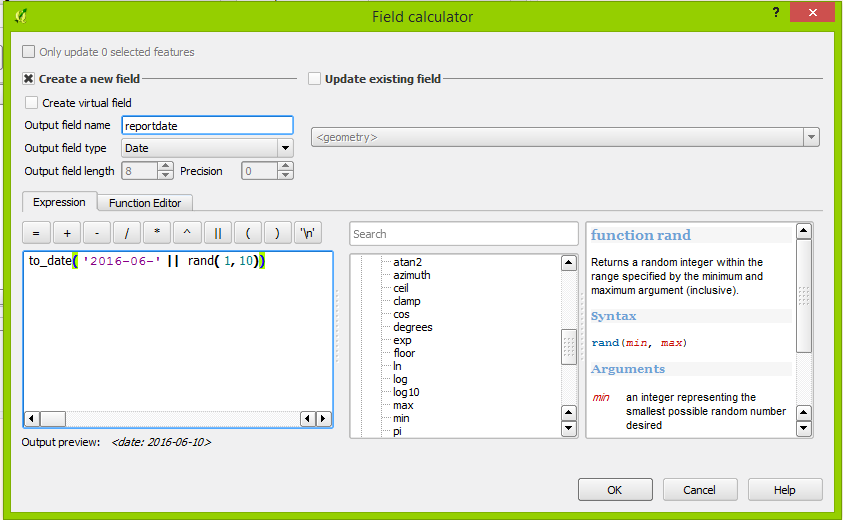
\includegraphics[width=12cm]{Images/field_calc.png}
	\caption{Generating random dates}\label{fig:field_calc}
\end{figure}

To animate the change in time you will use a QGIS plugin called TimeManager. Go to menu \textit{Plugins:Manage and Install Plugins}. In the \textit{Search} field type \textit{TimeManager} and install the plugin that will be listed (Figure \ref{fig:time_manager1}). At the bottom of the QGIS window a new dock widget named \textit{Time Manager} should show up. Click on the \textit{Settings} button in that widget.

\begin{figure}[H]
	\centering
	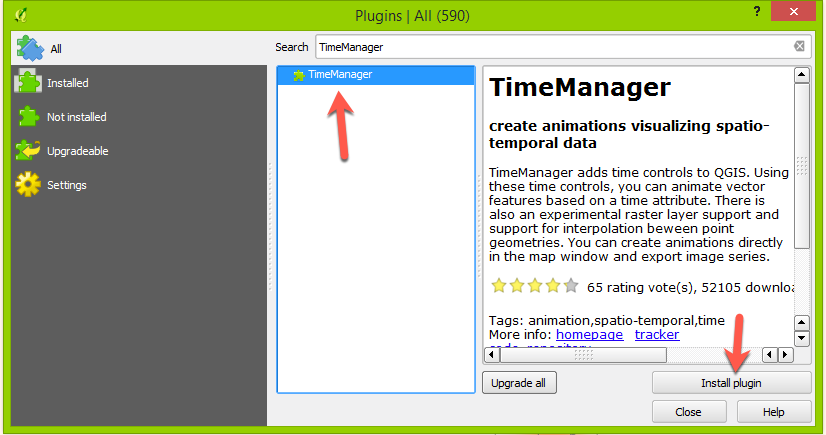
\includegraphics[width=12cm]{Images/time_manager1.png}
	\caption{Installing the TimeManager plugin}\label{fig:time_manager1}
\end{figure}

In the \textit{Time Manager Settings} dialog click on \textit{Add layer} and do the settings as shown in Figure \ref{fig:time_manager2}. In the main dialog for the settings do the changes as shown in Figure \ref{fig:time_manager3}.

\begin{figure}[H]
	\centering
	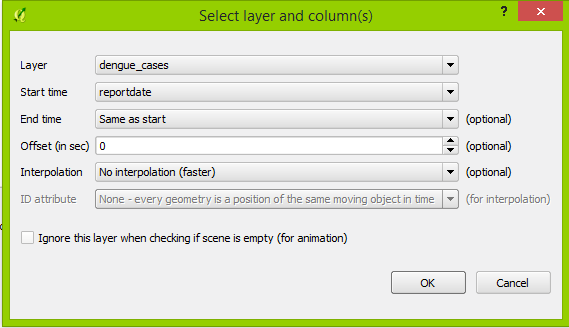
\includegraphics[width=8cm]{Images/time_manager2.png}
	\caption{Layer settings in Time Manager}\label{fig:time_manager2}
\end{figure}

\begin{figure}[H]
	\centering
	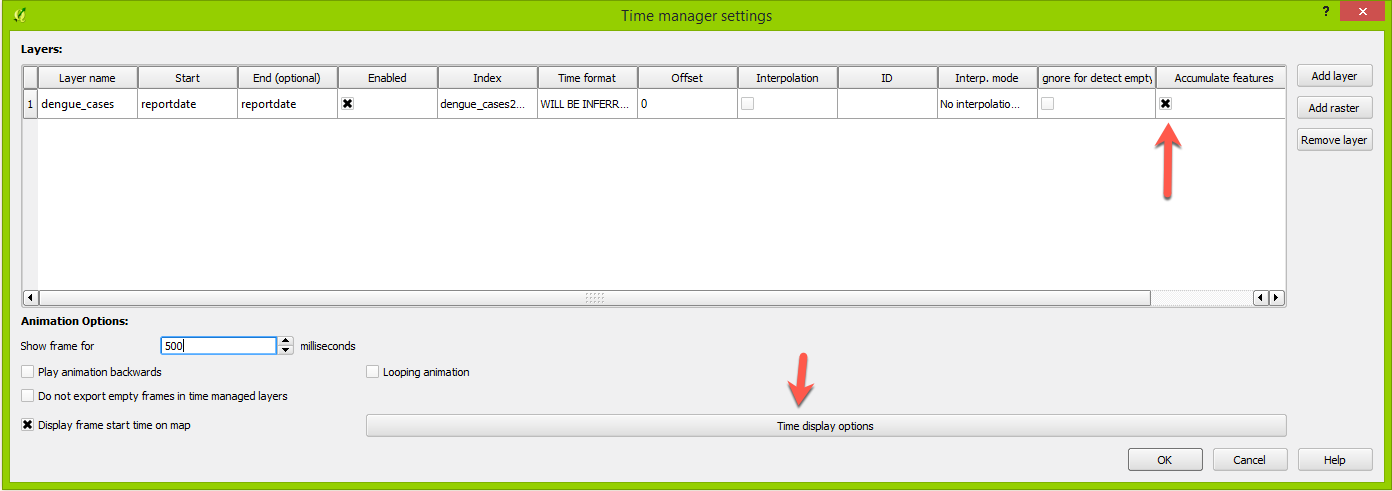
\includegraphics[width=12cm]{Images/time_manager3.png}
	\caption{Additional settings in Time Manager}\label{fig:time_manager3}
\end{figure}

Once done with these settings change the \textit{Time Frame Size} to \textit{1 day} on the \textit{Time Manager} dock widget. The day is the highest temporal resolution for the data you have. Finally click the \textit{Play} button to see the animation of the Dengue cases throughout time (Figure \ref{fig:time_manager4}).
	
\begin{figure}[H]
	\centering
	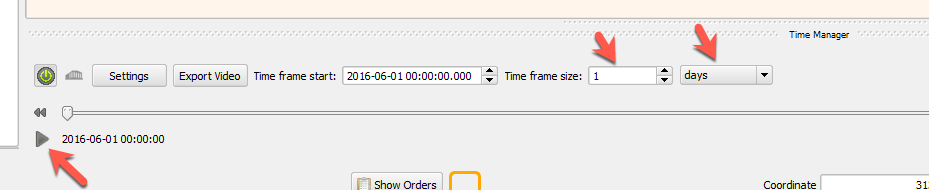
\includegraphics[width=12cm]{Images/time_manager4.png}
	\caption{Setting the time frame size}\label{fig:time_manager4}
\end{figure}	


\end{document}
